\begin{apendicesenv}

\partapendices

\chapter{Organização dos cabos da placa de condicionamento de sinais}

\section{Organização dos cabos}

Os cabos da placa dos sensores de tensão e dos sensores de corrente foram organizados conforme a Fig. \ref{fig:padrao_fios}.

\begin{figure}[!hbt]
        \begin{center}
        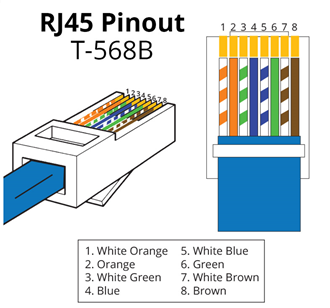
\includegraphics[width=5 cm, height=5cm]{figuras/T568B.png}
        \caption{Padrão de fios utilizado para o cabo das placas de aquisição}
        \label{fig:padrao_fios}
        \end{center}
\end{figure}

\subsection{Placa dos sensores de tensão}

Para placa dos sensores de tensão, pode-se realizar a crimpagem conforme a Fig. \ref{fig:padrao_fios}, porém tomando o cuidado para não utilizar os fios \textbf{laranja com branco} e \textbf{marrom com branco}. Logo, na hora de realizar a crimpagem, retirar esses fios. 

Não construir o cabo dos dois lados, somente crimpar do lado da placa dos sensores de tensão primeiramente, pois a ordem de conexão do lado da placa de condionamento é diferente do padrão da Fig. \ref{fig:padrao_fios}.

A organização para a placa dos sensores de tensão é:

\begin{itemize}
    \item Sensor LA20P 1 - Marrom 
    \item Sensor LA20P 2 - Verde 
    \item Sensor LA20P 3 - Azul 
    \item Sensor LA20P 4 - Laranja
    \item +15 V - Azul com branco
    \item -15 V - Verde com branco
\end{itemize}

\textbf{Atenção! Não utilizar os fios laranja com branco e marrom com branco.}

\subsection{Placa dos sensores de corrente}

Para a placa dos sensores de corrente, vale os mesmos procedimentos para a placa dos sensores de tensão. Tomar cuidado para não utilizar os fios \textbf{laranja com branco} e \textbf{marrom com branco}. Logo, na hora de realizar a crimpagem, retirar esses fios. Não construir o cabo dos dois lados, somente do lado da placa dos sensores de corrente. 

O mapeamento de sensores de corrente em cada fio é o seguinte:

\begin{itemize}
    \item Sensor LA55P 1 - Marrom 
    \item Sensor LA55P 2 - Verde 
    \item Sensor LA55P 3 - Azul 
    \item Sensor LA55P 4 - Laranja
    \item +15 V - Azul com branco
    \item -15 V - Verde com branco
\end{itemize}

\textbf{Atenção! Não utilizar os fios laranja com branco e marrom com branco.}

\subsection{Placa de Condionamento}

Para a placa de condionamento, utilizar a \textbf{Entrada 1} para o cabo dos sensores de corrente e a \textbf{Entrada 2} para o cabo dos sensores de tensão. 

A Entrada 1 está mapeada para as placas de aquisição de 1 a 4, e a Entrada 2 está mapeada para as placas de aquisição de 5 a 8.

Para a entrada 1 da placa de aquisição, os fios que vêm da placa dos sensores de corrente estão organizados da seguinte forma:

\begin{itemize}
    \item Placa 1 - Marrom (Sensor LA55P 1)
    \item Placa 2 - Verde (Sensor LA55P 2)
    \item Placa 3 - Azul (Sensor LA55P 3)
    \item Placa 4 - Laranja (Sensor LA55P 4)
\end{itemize}

Os fios azul com branco e verde com branco \textbf{devem ser invertidos} um com o outro baseado-se na organização da Fig. \ref{fig:padrao_fios}, pois do modo como estão, farão um curto-circuito na placa de aquisição.

Logo a sequência para a ponta do cabo na entrada da placa de aquisição, para o caso da placa dos sensores de corrente, é:

\textbf{laranja com branco - laranja - azul com branco - azul - verde com branco - verde - marrom com branco- marrom}

Não é necessário mais remover os fios laranja com branco e marrom com branco se estes já tiverem sido removidos anteriormente.

Para a Entrada 2, vale a mesma organização da Entrada 1. As placas de aquisição estão mapeadas da seguinte forma:

\begin{itemize}
    \item Placa 5 - Laranja (Sensor LA20P 4) 
    \item Placa 6 - Azul  (Sensor LA20P 3)
    \item Placa 7 - Verde (Sensor LA20P 2)
    \item Placa 8 - Marrom (Sensor LA20P 1)
\end{itemize}

Nenhuma alteração é nessária para a saída placa de aquisição de sinais. Pode-se crimpar o cabo conforme a Fig. \ref{fig:padrao_fios}. A saída de sinais da placa de aquisição de sinais tem a seguinte organização, supondo que o cabo crimpado baseia-se na Fig. \ref{fig:padrao_fios}:

\begin{itemize}
    \item Placa 1 - Azul com branco (Sensor LA55P 1)
    \item Placa 2 - Marrom com branco (Sensor LA55P 2)
    \item Placa 3 - Marrom (Sensor LA55P 4)
    \item Placa 4 - Verde (Sensor LA55P 3)
    \item Placa 5 - Azul (Sensor LA20P 4)
    \item Placa 6 - Laranja (Sensor LA20P 3)
    \item Placa 7 - Laranja com branco (Sensor LA20P 2)
    \item Placa 8 - Verde com branco (Sensor LA20P 1)
\end{itemize}

\end{apendicesenv}
